\documentclass[10pt]{beamer}

\newcommand{\lectnum}{L05}
\newcommand{\lecttitle}{Neural networks}

\usepackage{amsmath, amssymb, graphicx}
\usepackage[]{algorithm2e}
\usepackage{pdfpages}
\usepackage[british]{babel}

\hypersetup{colorlinks,linkcolor=,urlcolor=blue}
\newenvironment{titledslide}[1]{\begin{frame}\frametitle{#1}}{\end{frame}}

\mode<presentation>{\setbeamercovered{transparent}}

\setbeamertemplate{sidebar right}{}
\setbeamertemplate{footline}{%
\hfill\usebeamertemplate***{navigation symbols}
\hspace{0.4cm}\lectnum: \insertframenumber{}/\inserttotalframenumber \hspace*{0.4cm}}

\author{James Cussens}

\title{COMS30035, Machine learning:\\ \vspace{5pt} \lecttitle}

\institute{School of Computer Science\\University of Bristol}

\begin{document}
%%%%%%%%%%%%%%%%%%%%%%%%%%%%%%%%%%%%%%%%%%%%%%%%%%%%%%%%%%%%%%%%%%%%%%

\begin{frame}
  \titlepage
\end{frame}

%%%%%%%%%%%%%%%%%%%%%%%%%%%%%%%%%%%%%%%%%%%%%%%%%%%%%%%%%%%%%%%%%%%%%%

%%%%%%%%%%%%%%%%%%%%%%%%%%%%%%%%%%%%%%%%%%%%%%%%%%%%%%%%%%%%%%%%%%%%%%
\begin{titledslide}{Acknowledgement}

  \begin{itemize}
  \item These slides are adapted from ones originally created by
    \href{https://www.dpag.ox.ac.uk/team/rui-ponte-costa}{Rui Ponte
      Costa} and later edited by Edwin Simpson. 
  \end{itemize}
  
\end{titledslide}
%%%%%%%%%%%%%%%%%%%%%%%%%%%%%%%%%%%%%%%%%%%%%%%%%%%%%%%%%%%%%%%%%%%%%%
\begin{frame}[fragile]

  \frametitle{Textbooks}
We will follow parts of the Chapter 4 and 5 of the Bishop book:
\begin{itemize}
	\item Bishop, C. M., Pattern recognition and machine learning (2006). Available for free \href{https://www.microsoft.com/en-us/research/people/cmbishop/}{\underline{here}.}	\vspace{10pt}
\vspace{10pt}
\end{itemize}

\end{frame}
%%%%%%%%%%%%%%%%%%%%%%%%%%%%%%%%%%%%%%%%%%%%%%%%%%%%%%%%%%%%%%%%%%%%%%
\begin{frame}[fragile]
  
  \frametitle{Agenda}
  \begin{itemize}
  \item Perceptron
  \item Neural networks (multi-layer perceptron)
    \begin{itemize}
    \item Architecture
    \item The backpropagation algorithm
    \item Gradient descent
    \end{itemize}
  \end{itemize}
  See: \begin{small}[Chapter 5, Bishop]\end{small}

\end{frame}
%%%%%%%%%%%%%%%%%%%%%%%%%%%%%%%%%%%%%%%%%%%%%%%%%%%%%%%%%%%%%%%%%%%%%%          





\begin{frame}[fragile]
\frametitle{Perceptron -- a simplified neural network}



\begin{itemize}
	\item It is the very beginning of neural network models in ML! \vspace{3pt}\\
	\item It is directly inspired by how neurons process information: \vspace{3pt}\\	
	\centerline{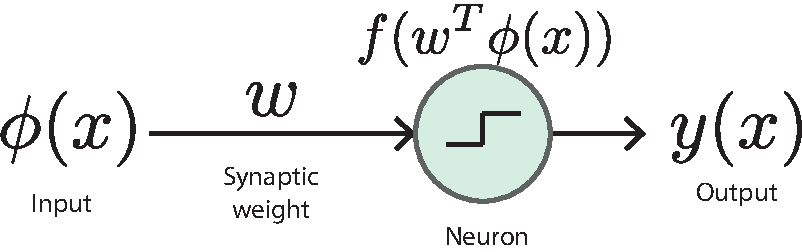
\includegraphics[scale=0.4]{../figures/Rosenblatt_neuron.pdf}}
\uncover<2->{	\item It is an example of a linear discriminant model given by $y(\bm{x}) = f(\bm{w}^T\phi(\bm{x}))$\\ 
	with a nonlinear \emph{activation function} $f(a) = \begin{cases}
+1, &a \geq 0 \\
-1, &a < 0
\end{cases} $}
\uncover<3->{
\item Here the target $t = \{+1, -1\}$.
\item And we aim to mimimise the following error $ - \mathlarger{\sum_{n=1}^N \bm{w}^T\phi_nt_n }$ \footnote{Intuitively we want to improve our chances of having $t_n = y_n = -1$ or $t_n = y_n = 1$, which will both decrease our error function.}}
\end{itemize}

\end{frame}



\begin{frame}[fragile]
\frametitle{Perceptron -- a simplified neural network}


\begin{example}
\centerline{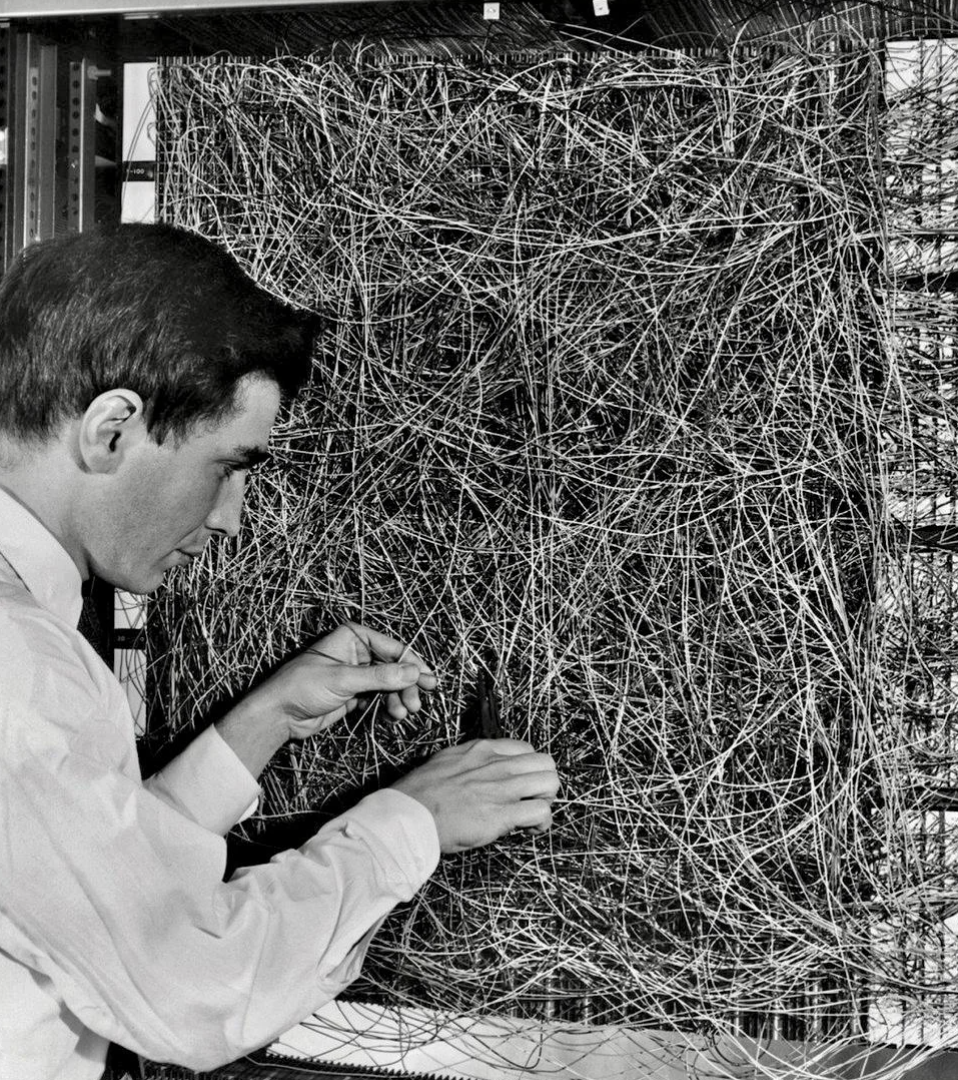
\includegraphics[scale=0.15]{../figures/Rosenblatt.png}}
\textbf{\textcolor{red}{The Perceptron of Rosenblatt (1962)}}\\
Perceptrons started the journey to the current \emph{deep learning} revolution!

Frank Rosenblatt used IBM and special-purpose hardware for a parallel implementation of perceptron learning. 

Marvin Minksy, showed that such models could only learn \emph{linearly separable problems}. 

However, this limitation is only true in the case of single layers!
\end{example}
{\fontsize{6}{6} \selectfont source: Bishop p193.}

\end{frame}


%
%\begin{frame}[fragile]
%\frametitle{Linear separability}
%
%\begin{example}
%To illustrate We generated data using two  for two classes . The main features are the petal and sepal size, samples below for 2 classes ($K=2$). \\
%	\begin{itemize}
%		\item \textcolor{darkgray}{$C = \{\text{iris setosa, iris versicolor}\}$
%		\item $x = \{ \text{petal size, sepal size} \}$}
%	\end{itemize}
%	
%\centerline{\includegraphics[scale=0.3]{../figures/iris_dataset_2classes.png}}
%\end{example}
%
%\end{frame}
%
%
%\begin{frame}[fragile]
%\frametitle{The Iris dataset}
%
%\begin{example}
%The iris dataset is one of the most popular datasets used in ML. The main features are the petal and sepal size, samples below for 2 classes ($K=2$). \\
%	\begin{itemize}
%		\item \textcolor{darkgray}{$C = \{\text{iris setosa, iris versicolor}\}$
%		\item $x = \{ \text{petal size, sepal size} \}$}
%	\end{itemize}
%	
%\centerline{\includegraphics[scale=0.3]{../figures/iris_dataset_2classes.png}}
%\end{example}
%
%\end{frame}


\begin{frame}[fragile]
\frametitle{Neural networks}

From a single layer perceptron:\\

	\centerline{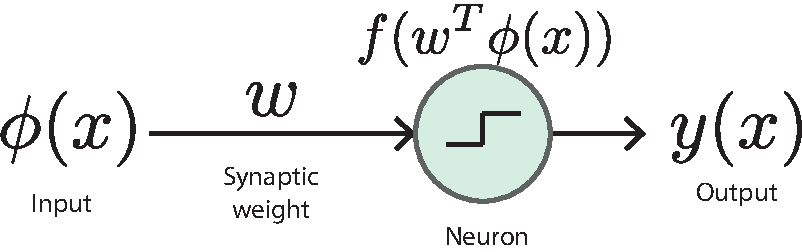
\includegraphics[scale=0.5]{../figures/Rosenblatt_neuron.pdf}}
	
%However these and other linear (or near-linear) models have limited expressibility due to the \emph{curse of dimensionality}.

\end{frame}


\begin{frame}[fragile]
\frametitle{Neural networks}

To a Multiple Layer Perceptron (MLP) \footnote{Although, we call it perceptron, it typically uses logistic sigmoid activation functions (continous nonlinearities), instead of step-wise discontinous nonlinearities.}:\vspace{5pt}\\

	\centerline{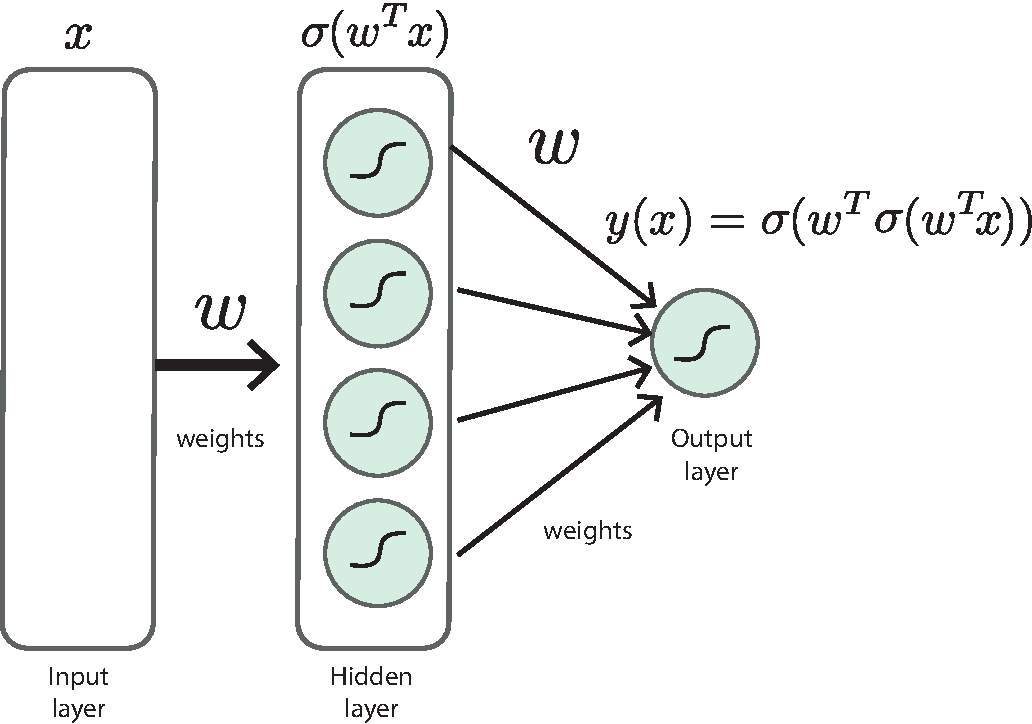
\includegraphics[scale=0.5]{../figures/MLP.pdf}}

\end{frame}


\begin{frame}[fragile]
\frametitle{Neural networks}


\begin{itemize}
	\item Neural networks are at heart composite functions of linear-nonlinear functions. 
	\item \textbf{Deep learning}\footnote{If you would like to learn more take our Applied Deep Learning unit in your 4th year.} refers to neural networks (or MLPs) with more than 1 hidden layer\\	
	\item They can be applied in any form of learning, but we will focus on \underline{supervised learning} and classification in particular\\	
\uncover<2->{	\item MLP recipe \footnote{Here we focus on simple feedforward nnets but the recipe is the same for any neural network.}:
	\begin{itemize}	
		\item Define architecture (e.g. how many hidden layers and neurons) \footnote{Note that this makes them parametric models.}
		\item Define cost function (e.g. mean squared error)
		\item Optimise network using backprop:
			\begin{enumerate}	
				\item Forward pass -- calculate activations; generate $y_k$
				\item Calculate error/cost function	
				\item Backward pass -- use backprop to update parameters
			\end{enumerate}	
	\end{itemize}}
\end{itemize}

\end{frame}



\begin{frame}[fragile]
\frametitle{Neural networks -- forward pass step-by-step}

\begin{enumerate}
	\item \small Calculate activations of the hidden layer $h$: $a_j = \mathlarger{\sum_{i=1}^D} w_{ji}^{(h)}x_i + w_{j0}^{(h)}$  [linear]
	\item \small Pass it through a nonlinear function: $z_j = \sigma(a_j)$ [nonlinear\footnote{In MLP we typically use sigmoid functions.}]
\uncover<2->{	\item \small Calculate activations of the output layer $o$: $a_k = \mathlarger{\sum_{j=1}^{hiddensize}} w_{kj}^{(o)}z_j + w_{k0}^{(o)}$  [linear]
	\item \small Compute predictions using a sigmoid: $y_k = \sigma(a_k)$ [nonlinear\footnote{For classification problems we use a sigmoid at the output, where each output neuron codes for one class.}]}
\uncover<3->{	\item \small All together: $y_k = \sigma \left( \mathlarger{\sum_{i=1}^D} w_{kj} \: \sigma \left(\mathlarger{\sum_{i=1}^D} w_{ji}x_i^{(h)} + w_{j0}^{(h)}\right) + w_{k0}^{(o)} \right)$}
\end{enumerate}

\end{frame}


\begin{frame}[fragile]
\frametitle{Neural networks -- backward pass}

\small We now need to optimise our weights, and as before we use derivatives to find a solution. Effectively backpropagating the output error signal across the network -- backpropagation algorithm.

\centerline{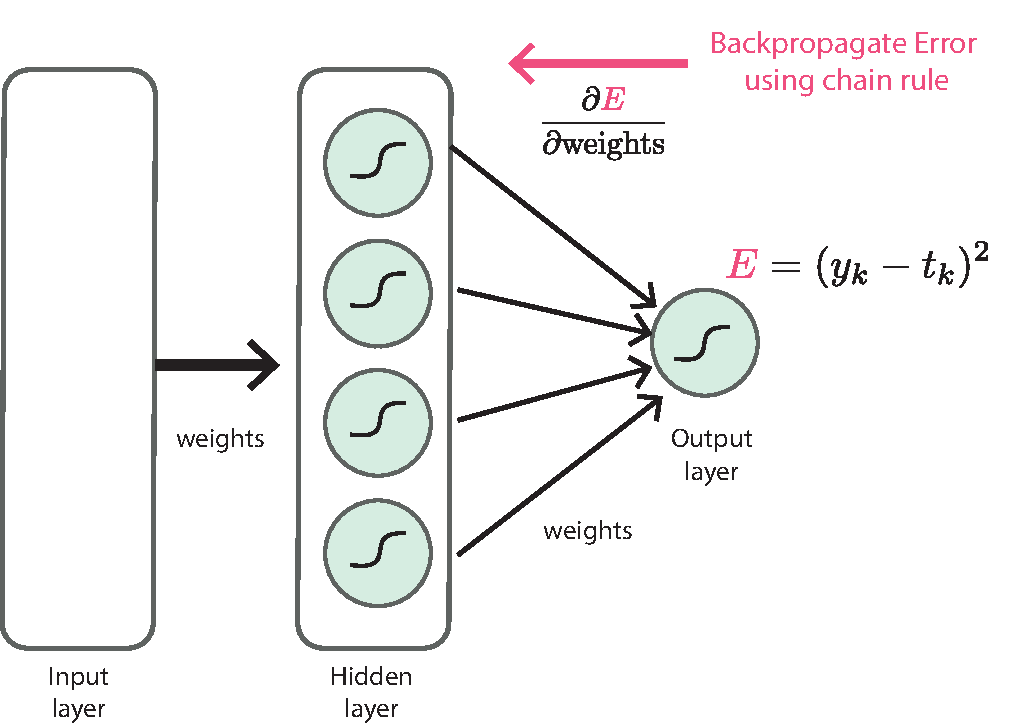
\includegraphics[scale=0.5]{../figures/MLP_back.pdf}}


\end{frame}


\begin{frame}[fragile]
\frametitle{Neural networks -- backward pass}

\small We now need to optimise our weights, and as before we use derivatives to find a solution. Effectively backpropagating the output error signal across the network -- backpropagation algorithm.

\begin{enumerate}
	\item \small Compute the error (or cost) function: e.g.: $E = \mathlarger{\frac{1}{2}\sum_{n=1}^N} (\bm{y(x_n,w}) - \bm{t_n})^2$
\uncover<2->{	\item \small Use the \emph{chain rule} to compute the gradients w.r.t. $\bm{w}$, $\frac{dE}{d\bm{w}}$
	\item \small For the output weights $w_{kj}$ we get:\\ $\mathlarger{\frac{\partial E}{\partial w_{kj}} = \frac{\partial E}{\partial y_{k}} \frac{\partial y_k}{\partial a_k} \frac{\partial a_k}{\partial w_{kj}} = \sigma'(y_n - t_n)z_j}$ \footnote{$\sigma '$ denotes the derivative of the sigmoid activation function.}}
\uncover<3->{	\item \small Whereas for the input weights $w_{ji}$ we get: \\$\mathlarger{\frac{\partial E}{\partial w_{ji}} = \frac{\partial E}{\partial y_{k}} \frac{\partial y_k}{\partial a_k} \frac{\partial a_k}{\partial z_{j}}  \frac{\partial z_j}{\partial a_j} \frac{\partial a_j}{\partial w_{ji}} = \sigma' (y_n - t_n) w_{kj}^T \sigma' x_i}$ \footnote{Note that the updates for the bias terms $w_0$ do not depend on the activity of the previous layer $z_j$ and $x_i$.}}
\end{enumerate}

\end{frame}



\begin{frame}[fragile]
\frametitle{Neural networks -- gradient descent \footnote{\tiny Its called descent because we are minimising the cost function, so descending on the function landscape, which can be quite hilly!}}

\small In many ML methods is common to iteratively update the parameters by descending the gradient. \vspace{10pt}\\

\centerline{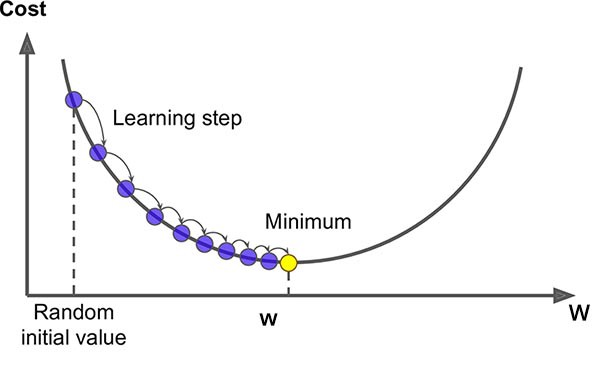
\includegraphics[scale=0.25]{../figures/grad_desc.jpeg}\footnote{\tiny Figure from \url{https://mc.ai/an-introduction-to-gradient-descent-2/}}}

\uncover<2->{In our neural network this means to update the weights using:

\begin{itemize}
	\item \small $w_{ji} = w_{ji} - \Delta w_{ji}$, where $\Delta w_{ji} = \sigma' (y_n - t_n) w_{kj}^T \sigma' x_i$
	\item \small $w_{kj} = w_{kj} - \Delta w_{kj}$, where $\Delta w_{kj} = \sigma'(y_n - t_n)z_j$
	\item \small This is often done in mini-batches -- using a small number of samples to compute $\Delta w$.
\end{itemize}}

\end{frame}




\begin{frame}[fragile]
\frametitle{Neural networks}

\begin{example}
Using sklearn we fitted a MLP classifier to the data: \vspace{5pt}\\	
\centerline{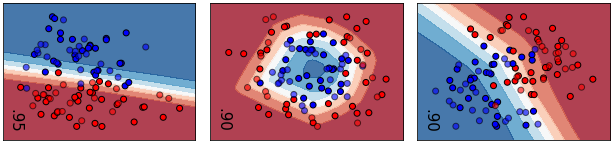
\includegraphics[scale=0.5]{../figures/nnet_class.png}}
\end{example}
\small An MLP with one hidden layer can perform well in nonlinear classification problems. 

However, because MLPs are highly flexible  they can easily \emph{overfit}. 

Solutions: \emph{early stopping} (stop when test performance starts decreasing) and \emph{regularisation} methods such as \emph{dropout} (randomly turn off units during training).
\end{frame}




\begin{frame}[fragile]
\frametitle{Classification methods -- overall comparison}

\centerline{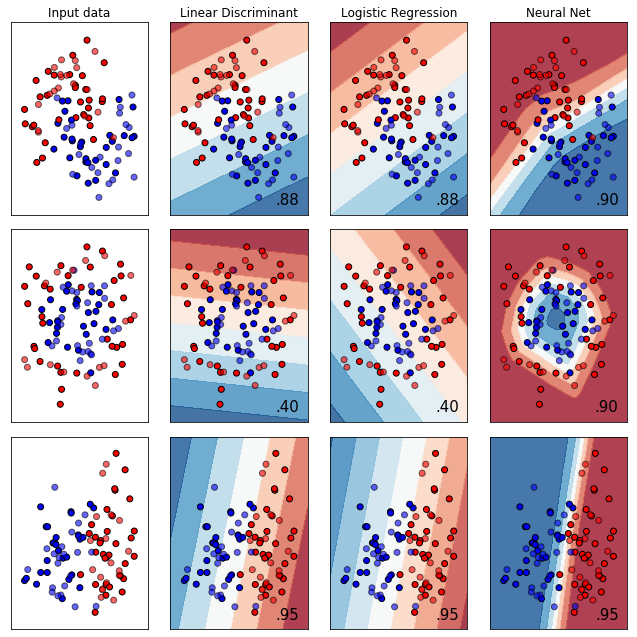
\includegraphics[scale=0.35]{../figures/classifiers_comparison_this.png}}

\end{frame}



\begin{frame}[fragile]
\frametitle{Classification methods -- overall comparison \small [including methods from the upcoming lectures]}

\centerline{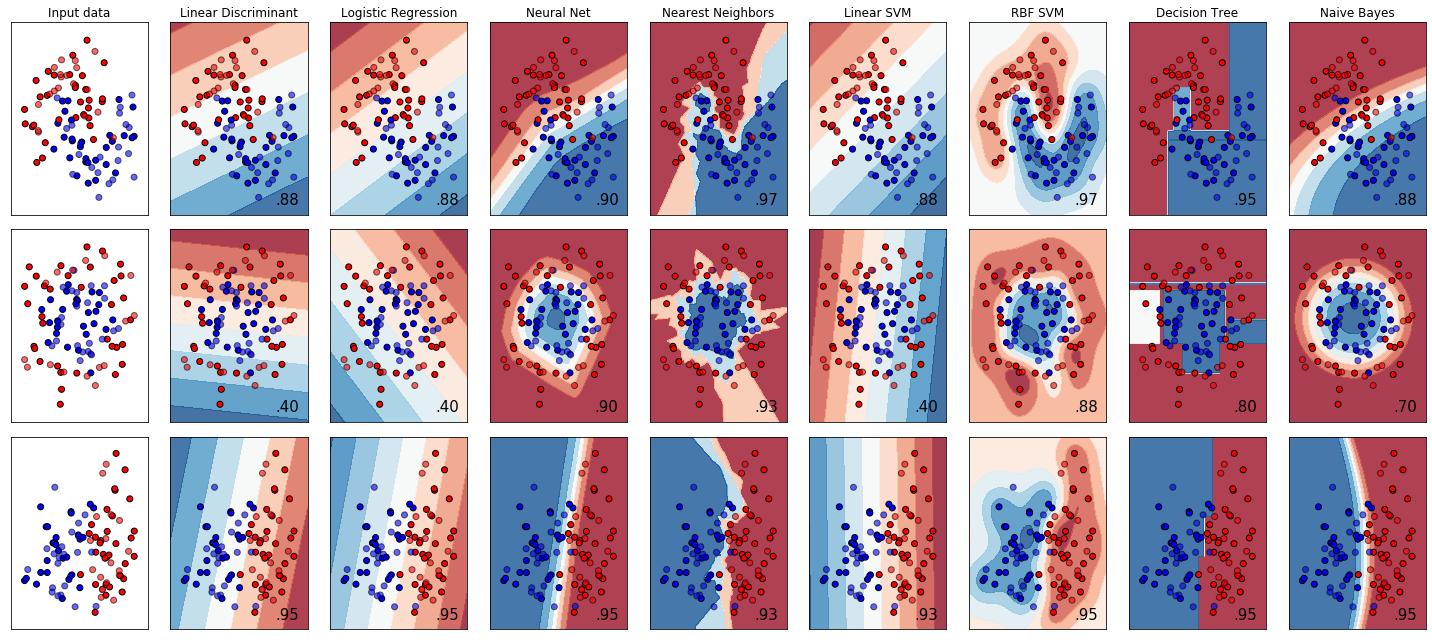
\includegraphics[scale=0.25]{../figures/classifiers_comparison.png}}
\end{frame}

\begin{frame}[fragile]
\frametitle{Quiz and video time!}
\centerline{
\includegraphics[scale=0.3]{../figures/BB.png}\vspace{10pt}}
\centerline{\begin{Large} Watch this \href{https://www.youtube.com/watch?v=cNxadbrN_aI}{\underline{very cool video}}  about the perceptron \footnote{Note the comment at the end -- it underlies all the recent successes using deep learning!}.\end{Large}}\vspace{10pt}
\begin{center}\begin{Large} Go to Blackboard unit page $\gg$ Quizzes $\gg$ Week 1 $\gg$ Classification and neural networks \end{Large}\end{center}\vspace{10pt}
\centerline{[Should take you less than 5 minutes]}
\end{frame}


\end{document}
